\lstset{language=Pascal,
        basicstyle=\footnotesize\ttfamily,
        breaklines=true,
        tabsize=2,
        numbers=left,
        numberstyle=\tiny,
        numbersep=7pt,
        showspaces=false,
        keywordstyle=\color{Blue}\textbf,
        commentstyle=\color{Red}\emph,
        showstringspaces=false,
        stringstyle=\color{BurntOrange}
        }
\section{Oprogramowanie sterownika}
W~niniejszym rozdziale opisane zostało oprogramowanie sterujące modelem. W~kolejnych podrozdziałach zostanie przedstawiona specyfikacja zewnętrzna oraz wewnętrzna. 

Stworzone przez autora oprogramowanie wraz ze~wszystkimi funkcjami systemowymi zajmują w~sterowniku 47428~kB z dostępnych 524288~kB. Zajętość pamięci dostępnej w~sterowniku obrazuje zrzut ekranu wykonany w~środowisku Step~7, widoczny na Rysunku~\ref{memory}.
%\begin{figure}[!htb] \centering 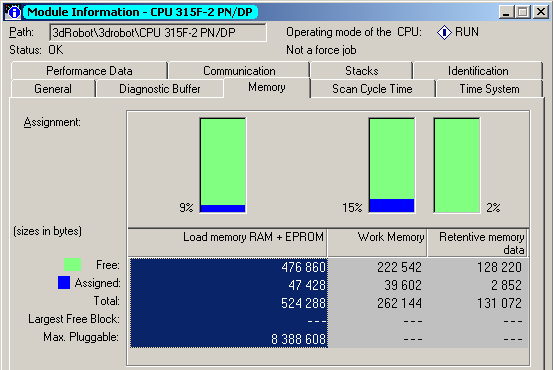
\includegraphics[width=0.6\textwidth]{obrazki/memory.PNG} \caption{Wykorzystanie pamięci sterownika} \label{memory} \end{figure}

\subsection{Specyfikacja zewnętrzna}
Specyfikacja zewnętrzna przedstawiona w dalszej części podrozdziału zawiera opis, jak korzystać z~oprogramowania wgranego do sterownika przez jego autora. Opisane zostało, jak ustawiać odpowiednie zmienne, aby~uzyskać żądany efekt.

Lista zmiennych wejściowych i wyjściowych wymieniana między sterownikiem a modelem została już opisana w~pierwszym rozdziale, w~Tablicach~\ref{in} oraz~\ref{out}. Pozostałe zmienne znajdują się w wewnętrznej pamięci sterownika.

Oprogramowanie może sterować modelem w~sposób automatyczny lub ręczny. Tryb automatyczny w~trybie obsługi magazynu zostanie opisany w podrozdziale 2.1.2. Tryb ręczny może być realizowany przy pomocy zadajnika podpiętego do sterownika lub przy pomocy przycisków umieszczonych na odpowiednim ekranie wizualizacji. W~trybie tym o~pracy robota decydujący jest stan przycisków. Dopuszczalne są wszystkie możliwe ruchy w~przedziale od wyłącznika krańcowego do wartości maksymalnej.

Sterowanie przy pomocy pilota podłączonego do sterownika odbywa się za pomocą 4~przycisków monostabilnych do załączania silników oraz 4~przełączników bistabilnych do wybierania kierunku. Podobne do sterowania pilotem jest sterowanie ręczne z~poziomu wizualizacji, polegające na odpowiednim modyfikowaniu bitów: M11.0~-~M11.7.

W automatycznym trybie pracy kluczową rolę odgrywają 4~zmienne: \emph{LiftEndPos}, \emph{GrabEndPos}, \emph{ArmEndPos} oraz \emph{RotateEndPos} typu INT, które wskazują na pozycje docelowe silników. Są one podawane do bloków FB1 odpowiadających kolejnym silnikom. O tym, czy wybrany silnik może się w~danym momencie poruszać czy nie decydują flagi odpowiednio ustawione przez blok FB9. 

Ważnym elementem jest kolejka obsługiwana w~trybie automatycznym. Indeksy przechowywane są w~przestrzeni od DB6.DBW0 do DB6.DBW202, a~związane z~nimi bezpośrednio zmienne typu bool - w przestrzeni od DB6.DBX202.0 do DB6.DBX216.0. Z kolejką tą związana jest dodatkowo zmienna \emph{CurrentIndex} określająca jej długość.

Kolejną przestrzenią adresową jest blok DB5, który jest reprezentacją w pamięci sterownika modelu magazynu i informacji o nim. Od adresu DB5.DBX0.0 znajduje się 26-elementowa tablica określająca zajętość poszczególnych komórek magazynu. Następnie od adresu DB5.DBW4 dostępna jest dwuwymiarowa tablica 26x3 przechowująca pozycję poszczególnych komórek magazynu. W~przestrzeni zaczynającej się pod adresem DB5.DBB160 znajduje się 26-elementowa tablica zmiennych typu DATE\_AND\_TIME przechowująca datę ostatniego dostępu do komórki. Dodatkowo w przestrzeni tej mamy dostępną pod adresem DB5.DBB368 zmienną przechowującą aktualną datę oraz godzinę w sterowniku, odświeżaną przy każdym przebiegu bloku OB1.

\subsection{Specyfikacja wewnętrzna}
Podrozdział specyfikacja wewnętrzna opisuje sposób rozwiązania przez autora kwestii sterowania modelem przy użyciu dostępnego na~stanowisku sterownika oraz poszczególnych trybów sterowania.
W~tworzeniu oprogramowania zostały wykorzystane następujące języki programowania:
\begin{itemize} 
\item język drabinkowy (Ladder), wykorzystany do stworzenia głównych elementów programu,
\item S7-SCL, który został zastosowany do korzystania z tablic. Niestety do korzystania z nich nie można zastosować języka LAD, ponieważ nie da się w~nim odwoływać do elementów tablicy przez indeksy będące zmiennymi, a~jedynie przez stałe. Po zapoznaniu się z~dokumentacją okazało się, że~taka możliwość istnieje w~języku STL, ale jest to metoda skomplikowana w~implementacji. Właśnie dlatego najlepszym i~najprostszym rozwiązaniem okazuję się S7-SCL, który jest kompilowany do kodu w~języku STL.
\end{itemize} 
Istotne fragmenty programu aplikacyjnego:
\begin{itemize} 
\item blok funkcyjny FB1 - blok sterujący pracą poszczególnych silników,
\item blok funkcyjny FB8 - blok zawierający implementację kolejki FIFO,
\item blok funkcyjny FB9 - blok analizujący stan modelu i ustawiający zmienne zezwalające na ruch silników,
\item blok funkcyjny FB10 - blok przetwarzający zadania z kolejki na odpowiednie dane (operuje na odpowiednich tablicach),
\item blok funkcyjny FB11 - blok zwracający indeks i zmienną bool najbliższego lub najdalszego elementu,
\item blok funkcyjny FB12 - blok zwracający indeks i zmienną bool najmłodszego lub najstarszego elementu.
\end{itemize} 
\indent
\indent Wszystkie wymienione bloki zostaną szczegółowo opisane w kolejnych podrozdziałach.
\vspace*{-9mm}
%dokładniejszy opis poszczególnych bloków w kolejnych podrozdziałach
\subsubsection{Blok FB1}
Najważniejszą częścią oprogramowania jest blok funkcyjny~FB1. Wszystkie zmienne wejściowe oraz wyjściowe dla tego bloku zostały zebrane w Tablicah~\ref{fb1datain}~oraz~\ref{fb1dataout}. Do~działania wykorzystuje~on zestaw danych wewnętrznych. Jako parametry wejściowe bloku, oprócz zmiennych z~modułu~I/O sterownika, podajemy typ aktualnego trybu, maksymalną dopuszczalną wartość wewnętrznego licznika, pozycję docelową w~trybie automatycznym oraz~zmienne \emph{Enable} i \emph{ResetSequence}. Ostatnie dwie zmienne odpowiadają za~to, aby~ruchy w~trybie automatycznym i resetowanie wykonywane były w~odpowiedniej kolejności. Na~wyjściu mamy tylko połączenia dla~zmiennych z~tablicy Symbols oraz~flagę osiągnięcia pozycji docelowej przez dany silnik.

\begin{table}[!htb]
\begin{center}
\begin{tabular}{|c|c|p{8.9cm}|}\hline
Nazwa & Typ & Opis  \\
zmiennej &  zmiennej &   \\\hline
StopSensor & Bool & Sygnał z odpowiedniej krańcówki \\\hline   
EngineCounter & Bool & Sygnał z impulsatora obrotów\\\hline   
CounterMax\_I & Int & Maksymalna wartość licznika typu Int \\\hline   
EndPosition & Int & Pozycja docelowa \\\hline   
Automat & Bool & Tryb automatyczny \\\hline   
ManualWorkDirection & Bool & Start w trybie ręcznym z                                   pilota \\\hline   
ManualWorkStart & Bool & Start w trybie ręcznym z                               wizualizacji \\\hline   
VisualWorkDirection & Bool & Kierunek w trybie ręcznym                                   z pilota \\\hline   
VisualWorkStart & Bool & Kierunek w trybie ręcznym                               z wizualizacji \\\hline   
CounterForState & Counter & Licznik wewnętrzny z aktualną pozycją \\\hline   
Enable & Bool & Sygnał zezwalający na                                                  inkrementację \\\hline   
ResetSequence & Bool & Zmienna pozwalająca na sekwencyjny reset \nobreak{modelu} \\\hline   
VisualPilot & Bool & Zmienna określająca tryb pracy manualnej \break z~pilota~lub wizualizacji \\\hline   
\end{tabular}
\end{center}
\vspace*{-6mm}
  \caption{Zmienne wejściowe do bloku FB1}
	\label{fb1datain}
\end{table}

\begin{table}[!htb]
\begin{center}
\begin{tabular}{|c|c| p{10cm} |}\hline
Nazwa & Typ & Opis  \\
zmiennej &  zmiennej &   \\\hline
EngineOnOff & Bool & Włączenie/wyłączenie                             silnika \\\hline   
EngineDirection & Bool & Kierunek pracy silnika \\\hline   
MinValue & Bool & Sygnał osiągnięcia                           minimum \\\hline   
MaxValue & Bool & Sygnał osiągnięcia                           maksimum \\\hline   
ReachPosition & Bool & Sygnał osiągnięcia                                pozycji docelowej \\\hline   
ResetFinish & Bool & Sygnał zakończenia                                resetu danego silnika \\\hline   
\end{tabular}
\end{center}
\vspace*{-6mm}
  \caption{Zmienne wyjściowe z bloku FB1}
	\label{fb1dataout}
\end{table}

Blok FB1 jest wywoływany w bloku OB1 z~odpowiednimi parametrami, niezależnie dla poszczególnych 4~silników. Przykładowe wywołanie znajduje się na Rysunku~\ref{ob1}. Na rysunku łatwo można zaobserwować, że do bloku podane są wszystkie niezbędne informacje dla danego silnika oraz 2~wspólne dla wszystkich silników sygnały informujące o~aktualnym trybie pracy modelu.
%\begin{figure}[!htb] 	\centering 	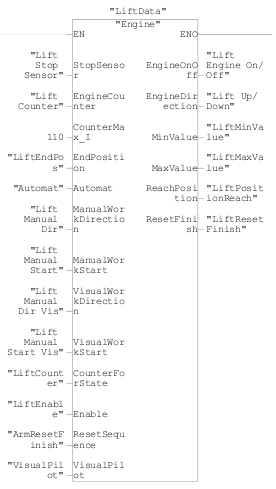
\includegraphics[width=0.58\textwidth]{obrazki/ob1.png} 	\caption{Przykładowe wywołanie FB1 w OB1 dla silnika Lift} \label{ob1} \end{figure} 

Istotnymi fragmentami bloku FB1 są 3~gałęzie programu: licznik wewnętrzny, decyzja o~kierunku oraz decyzja o~załączeniu.
Bardzo istotnym warunkiem wpływającym na pracę silnika jest jego położenie. Jeśli silnik osiąga wartość maksymalną lub minimalną to przerywa swoją pracę. Warunkiem koniecznym do określenia tej pozycji jest wykorzystanie licznika do zliczania impulsów z~modelu i~jego odpowiednia inkrementacja lub dekrementacja. Tak działający licznik przedstawia Rysunek~\ref{licznik}.
%\begin{figure}[!htb] 	\centering 	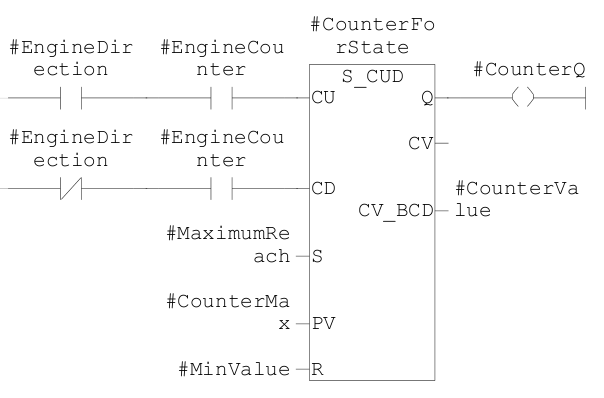
\includegraphics[width=0.5\textwidth]{obrazki/fb1licznik.png} 	\caption{Licznik wewnętrzny dla silnika w bloku FB1} \label{licznik} \end{figure} 

Decyzja dotycząca kierunku jest podejmowana zależnie od trybu pracy, co zaobserwować można na Rysunku~\ref{kierunek}. W~przypadku trybu automatycznego decydująca jest bieżąca pozycja oraz pozycja docelowa. Kierunek jest ustawiany tak, aby załączony silnik zmierzał do~pozycji docelowej. W~przypadku trybów manualnych decydujące są stany przycisków przy sterowaniu z~pilota lub zmienne przy sterowaniu z~wizualizacji. Jeżeli została podjęta decyzja o~załączeniu silnika to stan przycisku (zmiennej) jest wpisywany do zmiennej statycznej \emph{EngineDirectionManual}, która jest następnie zsumowana logicznie ze zmienną \emph{EngineDirectionAuto}, dając w~wyniku decyzję o~kierunku.
%\begin{figure}[!htb] 	\centering 	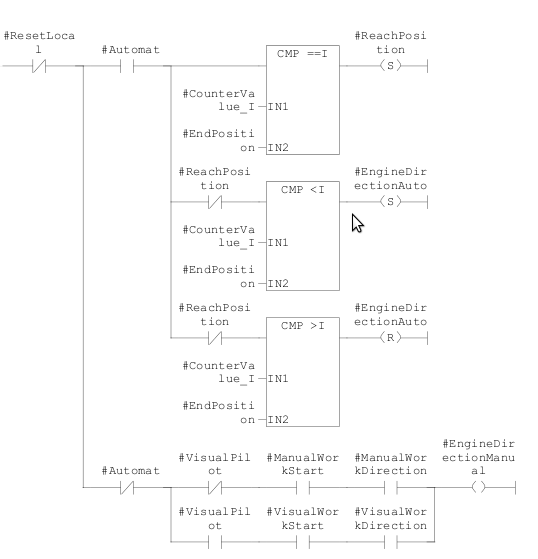
\includegraphics[width=0.66\textwidth]{obrazki/fb1kierunek.png} \caption{Fragment bloku FB1 wybierający kierunek pracy silnika} \label{kierunek} \end{figure} 

Część decydująca o~załączeniu silnika jest bardzo rozbudowana. Jest to przykład załączenia z~podtrzymaniem. Zależnie od trybu pracy sprawdzane są inne warunki. W~przypadku trybu automatycznego ważna jest zmienna \emph{Enable}, która decyduje o~załączeniu wybranego silnika, co pozwala na częściową pracę sekwencyjną. Silnik pracuje w~kierunku krańcówki aż do~jej osiągnięcia, a w~kierunku od krańcówki aż~do osiągnięcia swojego maksimum, chyba że~wcześniej zostanie osiągnięta pozycja docelowa. W~ręcznych trybach pracy głównym warunkiem decydującym o~załączeniu zależnie od kierunku są wartość maksymalna licznika lub krańcówka. Wspólnym dla obu trybów warunkiem pozwalającym zatrzymać pracę silnika jest ustawienie zmiennej \emph{EmergencyStop} na wartość \emph{true}. Tą rozbudowaną i skomplikowaną gałąź prezentuje Rysunek~\ref{onoff}.
%\begin{figure}[!htb] 	\centering 	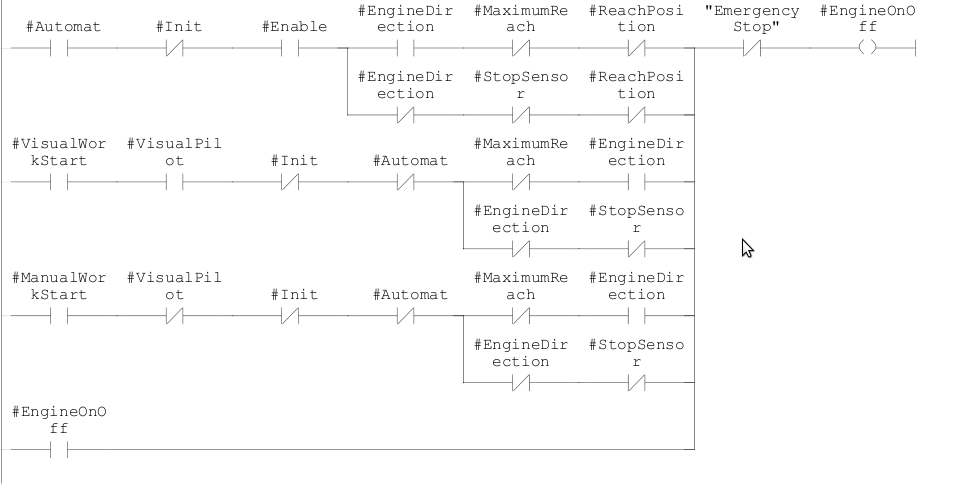
\includegraphics[width=0.95\textwidth]{obrazki/fb1wlwyl.png} 	\caption{Fragment bloku FB1 decydujący o załączeniu silnika} \label{onoff} \end{figure} 

\subsubsection{Blok FB8}
W trybie automatycznym podczas obsługi magazynu praca odbywa się na zasadzie zadań do wykonania. Na zadanie takie składa się indeks komórki w magazynie oraz zmienna typu bool, która decyduje o ruchu chwytaka (zaciskanie lub zwalnianie). Indeks jest następnie przetwarzany w odpowiednim bloku na położenie komórki w modelu magazynu. 

Bardzo ważnym blokiem funkcyjnym jest blok zarządzający kolejką zadań do wykonania w trybie automatycznym. Na wejściu znajdują się: dodawany do kolejki indeks oraz zmienna decydująca o zamknięciu lub otwarciu chwytaka. Na wyjściu mamy zmienne takie same jak na wejściu, ale przepuszczone już przez kolejkę. Zmienne wejściowo-wyjściowe to 2~flagi żądania, odpowiednio: dodania do kolejki lub pobrania z niej elementu oraz 2~flagi potwierdzające wykonanie żądania. Dodatkowo w~bloku tym występuje zmienna wewnętrzna stanowiąca indeks w~tablicy. 
\newpage
\begin{lstlisting}[caption={FB8 - Zarządzanie kolejką}]
FUNCTION_BLOCK FB8

VAR_INPUT
    AddedBool: BOOL;
    AddedIndex: INT;
END_VAR     

VAR_OUTPUT 
    WarehouseBool: BOOL;
    WarehouseIndex: INT;
END_VAR  

VAR_IN_OUT
    Request: BOOL;
    Add: BOOL;
    RequestAck: BOOL;
    AddAck: BOOL;
END_VAR  

VAR
    Index: INT ;
END_VAR

BEGIN
IF Add = true & Queue.CurentIndex <= 100 THEN
    IF AddedIndex >= 0 AND AddedIndex < 26 THEN
        Queue.QueueIndex[Queue.CurentIndex] := AddedIndex;
        Queue.QueueBool[Queue.CurentIndex] := AddedBool;
        Queue.CurentIndex := Queue.CurentIndex + 1;
        Add := false;
        AddAck := true;
    ELSE
        Error.IndexError := 'Indeks spoza zakresu';    
        Error.IndexErrorPres := true;
    END_IF;
ELSIF Queue.CurentIndex >= 100 THEN   
    Error.QueueError := 'Przepelniona Kolejka';
    Error.QueueErrorPres := true;    
END_IF;

IF Request = true & Queue.CurentIndex > 0 THEN
    IF Queue.QueueIndex[0] <> -1 THEN        
        WarehouseIndex := Queue.QueueIndex[0];
        WarehouseBool := Queue.QueueBool[0];
            FOR Index := 0 TO Queue.CurentIndex DO
                Queue.QueueIndex[Index] := Queue.QueueIndex[Index+1];
                Queue.QueueBool[Index] := Queue.QueueBool[Index+1]; 
            END_FOR;        
        Queue.QueueIndex[Queue.CurentIndex] := 0;
        Queue.QueueBool[Queue.CurentIndex] := false;
        Queue.CurentIndex := Queue.CurentIndex - 1;
        Request := false;
        RequestAck := true;
    ELSE
        Error.IndexError := 'Bledny indeks';    
        Error.IndexErrorPres := true;            
    END_IF;    
ELSIF Queue.CurentIndex = 0 THEN
    Request := false;   
    RequestAck := false;     
    Error.QueueError := 'Kolejka jest pusta';    
    Error.QueueErrorPres := true;
END_IF;
END_FUNCTION_BLOCK
\end{lstlisting}
\subsubsection{Blok FB9}
Kolejnym istotnym blokiem jest blok decydujący o~zezwoleniu na pracę poszczególnych silników, pozwalając przez to wykonywać ruchy ramienia w~odpowiedniej kolejności. Blok na wyjściu posiada 4~zmienne stanowiące właściwe zezwolenie na ruch. Decyzja jest podejmowana na podstawie położenia silnika Arm oraz osiągnięcia przez poszczególne silniki swoich pozycji docelowych.
\begin{lstlisting}[caption={FB9 - Zezwolenie na ruch}]
FUNCTION_BLOCK FB9

VAR_INPUT
    ArmCounterl: COUNTER;
END_VAR     

VAR_OUTPUT
    ArmEn: BOOL;
    LiftEn: BOOL;
    RotateEn: BOOL;
    GrabEn: BOOL;            
END_VAR     

BEGIN
    IF AutoTest THEN
        ArmEn := true;
        LiftEn := true;
        RotateEn := true;
        GrabEn := true;
    ELSE     
        IF ArmData.CounterValue_I <= 25 THEN
            ArmEn := true;
            LiftEn := true;
            RotateEn := true;
            GrabEn := false;
        ELSE
            IF LiftPositionReach  AND RotatePositionReach THEN        
                ArmEn := true;   
                LiftEn := false;
                RotateEn := false;
                GrabEn := false;  
            ELSE
                IF ArmData.CounterValue_I > 25 THEN
                    ArmEn := true;
                    LiftEn := false;
                    RotateEn := false;
                    GrabEn := false;
                else
                    ArmEn := false;   
                    LiftEn := true;
                    RotateEn := true;
                    GrabEn := false;              
                END_IF;
            END_IF;    
        END_IF;        
        IF LiftPositionReach & RotatePositionReach & ArmPositionReach THEN
            ArmEn := false;   
            LiftEn := false;
            RotateEn := false;
            GrabEn := true;    
        END_IF;    
    END_IF;           
END_FUNCTION_BLOCK
\end{lstlisting}

\subsubsection{Blok FB10}
Blok funkcyjny FB10 zarządza operacjami wykonywanymi na tablicach związanych z~obsługiwanym magazynem. Na~wejściu mamy zmienne stanowiące wyjście z~kolejki oraz zmienną określającą, że~wykonane zostało ostatnie podzadanie uruchomione przez ten blok. Na~wyjściu mamy zmienne określające, do jakich pozycji mają dojechać silniki. 

Zmienne wejściowo-wyjściowe to żądanie następnego zadania z~kolejki oraz potwierdzenie obsłużenia żądania przez kolejkę. Zmienna tymczasowa jest to wartość zwrócona przez funkcję systemową odczytu bieżącej daty oraz godziny. Zmienna wewnętrzna \emph{DoneCount} przechowuje informację o tym, ile podzadań zostało wykonanych. 
\begin{lstlisting}[caption={FB10 - Operacje na tablicah}]
FUNCTION_BLOCK FB10

VAR_INPUT
    Done: BOOL;
    WarehouseIndex: INT;
    WarehouseBool: BOOL;
END_VAR 

VAR_OUTPUT
    ArmTo: INT;
    LiftTo: INT;
    RotateTo: INT;
    GrabTo: INT;            
END_VAR

VAR_IN_OUT
    NextRequest: BOOL;
    NextRequestACK: BOOL;
END_VAR  
 
VAR_TEMP
    SFC1_Ret_val: INT;    
END_VAR

VAR
    DoneCount: INT;
    LoadNext: BOOL;
END_VAR
    
BEGIN

IF NextRequestACK = true THEN
    NextRequest := false;
    NextRequestACK := false;
    DoneCount := 0;    
    ArmTo := 22;
    IF WarehouseBool THEN
        LiftTo := Warehouse.WarehousePosition[WarehouseIndex, 2];    
    ELSE 
        LiftTo := Warehouse.WarehousePosition[WarehouseIndex, 2]-3;
    END_IF;  
    RotateTo := Warehouse.WarehousePosition[WarehouseIndex, 3];
    LoadNext := true;
END_IF;

IF DoneCount = 1 THEN
    ArmTo := Warehouse.WarehousePosition[WarehouseIndex, 1];
    IF WarehouseBool THEN
        LiftTo := Warehouse.WarehousePosition[WarehouseIndex, 2];    
    ELSE 
        LiftTo := Warehouse.WarehousePosition[WarehouseIndex, 2]-3;
    END_IF;        
    RotateTo := Warehouse.WarehousePosition[WarehouseIndex, 3];
    GrabTo := BOOL_TO_INT(WarehouseBool) * 19;
END_IF;
    
IF DoneCount = 2 THEN
    Warehouse.WarehouseBool[WarehouseIndex] := NOT WarehouseBool;
    SFC1_Ret_val := SFC1(CDT := Warehouse.WarehouseDateTime[WarehouseIndex]);
    DoneCount := 0;
    IF Queue.CurentIndex > 0 THEN
        NextRequest := true;
        LoadNext := false;
    ELSE
        Error.QueueError := 'Kolejka jest pusta';  
    END_IF;
END_IF;

IF Done = true & LoadNext THEN
    DoneCount := DoneCount + 1;    
END_IF;       
END_FUNCTION_BLOCK
\end{lstlisting}
\subsubsection{Blok FB11}
Blok FB11 w wyniku działania zwraca indeks komórki w magazynie oraz powiązaną z~nim zmienną typu bool, które pozwalają wybrać najdalej lub najbliżej położony element. Wskazuje on pustą lub zajętą komórkę magazynu, zależnie od zmiennych wejściowych. Zależnie od wartości zmiennej \emph{FarNear} wybierana jest najdalej lub najbliżej położona komórka, natomiast zmienna \emph{BoolGrab} decyduje o~tym, czy szukamy wolnej czy zajętej komórki magazynu. 

W wyniku działania blok ustawia na wyjściu zmienne związane z~wybraną komórką magazynu oraz flagę żądania dodania uzyskanego wyniku do kolejki zadań. Zmienna \emph{MyEn} decyduje o tym, czy ten blok zostaje aktywowany czy nie. Zmienna index jest zmienną wewnętrzną wykorzystywaną w~pętlach FOR.
\begin{lstlisting}[caption={FB11 - Funkcja wybiera najdalszą lub najbliższą komórkę}]
FUNCTION_BLOCK FB11

VAR_INPUT
    FarNear: BOOL;
END_VAR 

VAR_OUTPUT
    IndexSel: INT;
    AddQueue: BOOL;
END_VAR
 
VAR_IN_OUT
    MyEn: BOOL;
    BoolGrab: BOOL;
END_VAR  

VAR
    Index: INT;
END_VAR    
    
BEGIN
IF MyEn = true THEN    
    IF FarNear = true & BoolGrab = true THEN    
        FOR Index := 1 TO 24 DO
            IF Warehouse.WarehouseBool[Index] = true THEN
                IndexSel := Index;
                EXIT;
            ELSE
                IndexSel := -1;                
            END_IF;
        END_FOR;        
    END_IF;
    
    IF FarNear = false & BoolGrab = true THEN
        FOR Index := 24 TO 1 BY -1 DO
            IF Warehouse.WarehouseBool[Index] = true THEN
                IndexSel := Index;
                EXIT;
            ELSE
                IndexSel := -1;                                
            END_IF;            
        END_FOR;
    END_IF;
    
    IF FarNear = true & BoolGrab = false THEN
        FOR Index := 1 TO 24 DO
            IF Warehouse.WarehouseBool[Index] = false THEN
                IndexSel := Index;
                EXIT;
            ELSE
                IndexSel := -1;                                                
            END_IF;            
        END_FOR;
    END_IF;
    
    IF FarNear = false & BoolGrab = false THEN
        FOR Index := 24 TO 1  BY -1 DO
            IF Warehouse.WarehouseBool[Index] = false THEN
                IndexSel := Index;
                EXIT;
            ELSE
                IndexSel := -1;                                                
            END_IF;            
        END_FOR;
    END_IF;   
    MyEn := false;
    AddQueue := true;
END_IF;       
END_FUNCTION_BLOCK
\end{lstlisting}
\subsubsection{Blok FB12}
Blok FB12 w wyniku działania zwraca indeks komórki w magazynie oraz powiązaną z~nim zmienną typu bool, które pozwalają wybrać najstarszy lub najmłodszy element tablicy. Wskazuje on zajętą komórkę magazynu. Zależnie od wartości zmiennej \emph{SmallestGreatest} wybierana jest najmłodsza lub najstarsza zajęta komórka. 

W wyniku działania blok ustawia na wyjściu zmienne związane z~wybraną komórką magazynu oraz flagę żądania dodania uzyskanego wyniku do kolejki zadań. Zmienna \emph{MyEn} decyduje o~tym, czy ten blok zostaje aktywowany czy nie. Zmienna index jest zmienną wewnętrzną wykorzystywaną w~pętlach FOR. \emph{IndexTemp} jest zmienną pomocniczą stanowiącą tymczasowy indeks przy wybieraniu elementu końcowego.
\begin{lstlisting}[caption={FB12 - Funkcja wybiera najmłodszą lub najstarszą zajętą komórkę}]
FUNCTION_BLOCK FB12

VAR_INPUT
    SmallestGreatest: BOOL;
END_VAR 

VAR_OUTPUT
    IndexSelected: INT;
    BoolSelected: BOOL;
    AddQueue: BOOL;    
END_VAR
 
VAR_IN_OUT
    MyEn: BOOL;
END_VAR  
 
VAR
    Index: INT;
END_VAR
    
VAR_TEMP
    IndexTemp: INT;
END_VAR 
       
BEGIN
IF MyEn = true THEN    
    
    IF SmallestGreatest = false THEN    
        FOR Index := 1 TO 24 DO        
            IF Warehouse.WarehouseBool[Index] = true AND FC28(DT1 := Warehouse.WarehouseDateTime[Index], DT2 := DT#1990-01-01-12:00:00.00) THEN
                IndexTemp := Index;
                EXIT;
            ELSE
                IndexTemp := -1;
            END_IF;
        END_FOR;  
        IF IndexTemp <> -1 THEN                   
            FOR Index := 1 TO 24 DO        
                IF Warehouse.WarehouseBool[Index] = true then
                    IF FC14(DT1 := Warehouse.WarehouseDateTime[Index], DT2 := Warehouse.WarehouseDateTime[IndexTemp]) THEN
                        IndexTemp := Index;            
                    END_IF;
                END_IF;
            END_FOR;        
        END_IF;           
    END_IF;
    
    IF SmallestGreatest = true THEN
        FOR Index := 1 TO 24 DO        
            IF Warehouse.WarehouseBool[Index] = true AND FC28(DT1 := Warehouse.WarehouseDateTime[Index], DT2 := DT#1990-01-01-12:00:00.00) THEN
                IndexTemp := Index;
                EXIT;
            ELSE
                IndexTemp := -1;
            END_IF;
        END_FOR;      
        IF IndexTemp <> -1 THEN                   
            FOR Index := 1 TO 24 DO
                IF Warehouse.WarehouseBool[index] = true then        
                    IF FC23(DT1 := Warehouse.WarehouseDateTime[Index], DT2 := Warehouse.WarehouseDateTime[IndexTemp]) THEN
                        IndexTemp := Index;
                    END_IF;            
                END_IF;            
            END_FOR;
        END_IF;            
    END_IF;
    MyEn := false;
    IndexSelected := IndexTemp;
    BoolSelected := true;
    AddQueue := true;
END_IF;    
END_FUNCTION_BLOCK
\end{lstlisting}
